\chapter{Analysis of processing results}
\label{analysis_processing}
In this chapter the result of the data processing will be evaluated. Starting with the evaluation processing, which clusters the FCD, forms congestion events, finds adjacent incident and exports a list of congestion-incident matched. The second section will elaborate on the results of the correlation processing and use the results for a further analysis of relations.

\section{Evaluation Processing}
The results of the clustering and matching algorithm where visually reviewed to verify the performance. Thought iterative adjustments of the input parameters the clustering and matching algorithm where calibrated to a sufficient representation level (see final input parameters in \autoref{methodology_detection} and \autoref{methodology_matching}).

\todo{Add Figures of clustering as proof} 

\section{Correlation Processing}
\label{analysis_processing_evaluation}
The resulting datasets created by the evaluation tool (see section \autoref{methodology_detection} \autoref{methodology_matching} and \autoref{methodology_data_processing}), tasked with the detection and clustering of jams and search for adjacent incidents, are then processed by the correlation tool (\autoref{methodology_correlation_processing}). The correlation tool calculates multiple matrix tables with the correlation effect size, correlation significance and used correction coefficient for all variable combinations. From these tables and interpretation guidelines defined in \autoref{correlation_coefficient_types} for each coefficient type, we can deviated the strength of correlation and significance (see \autoref{correlation_significance}) for each combination. In the case of correlated and significant variables, it still needs to be determined what the found correlation predicates. This is done via the Post Hoc test, defined in \autoref{correlation_posthoc}.

\todo{Short explnation of Post Hoc}
All groups, where the $p$-value is below $\alpha=.05$, have significant differences.

\begin{table}[ht]
	\centering
	\begin{tabular}{r|c|c|c}  
		\toprule
		Coefficient & Weak 	& Moderate 	& Strong \\
		\midrule
		$r$ 		& .30	& .50		& .80 \\
		$\eta$ 		& < .06 & .06		& .14 \\
		$r_{pq}$	& < .30	& .30		& .50 \\
		$\tau$ 		& < .30	& .30		& .50 \\
		$V$ 		& < .30	& .30		& .40 \\
		\bottomrule
	\end{tabular}
	\caption{Correlation effect size interpretation for coefficient $r$,$\eta$,$r_{pq}$,$\tau$ and $V$}
	\label{tbl:correlation_interpretation_guidelines}
\end{table}

To recap \autoref{correlation_coefficient_types}, \autoref{tbl:correlation_interpretation_guidelines} shows the guidelines for a weak, moderate and strong correlation effect size of the coefficients $r$,$\eta$,$r_{pq}$,$\tau$ and $V$.

% -----------------------------------
% -------- BAYSIS - Matched ---------
% -----------------------------------
\subsection{Accident - Congestion Matched Complete}
\label{analysis_processing_correlation}
The correlation matrix table for the congestion-accident matched dataset (see \autoref{table:appendix_correlation_matrix_matched_cramers}) is visual presented in \autoref{img:correlation_matrix_matched_cramers} showing the the correlation of each variable combination. When visual analyzing \autoref{img:correlation_matrix_matched_cramers} and checking the guidelines for a strong correlation in reference to the applied coefficient (identifiable with \autoref{table:appendix_coefficient_matrix_matched}) we get a list of strongly correlated variable combinations (see \autoref{tbl:correlation_list_baysis_matched})

\begin{table}[ht]
	\centering
	\begin{tabular}{c|l}  
		\toprule
		Category & Strong \\
		\midrule
		Strasse & TMax, TAvg, SMax, SAvg, TDist, SDist, Cov \\ 
 		Kat & TMax, TAvg, SAvg, TDist \\ 
 		Typ & TDist, Cov \\
 		%Betei & & \\
 		UArt1 & SAvg, TDist, Cov \\
 		%UArt2 & & \\
 		AUrs1 & SAvg, TDist, SDist, Cov, TLHGV \\
 		%AUrs2 & & \\
 		AufHi & TMax, TAvg, TDist, Cov \\
 		%Alkoh & & \\
 		%Char1 & & \\
 		%Char2 & & \\
 		%Bes1 & & \\
 		Lich1 & Cov \\
 		Lich2 & Cov \\
 		Zust1 & Cov \\
 		%Zust2 & & \\
 		%Fstf & & \\
 		WoTag & Cov \\
 		%FeiTag & & \\
		Month & Cov \\
		\bottomrule
	\end{tabular}
	\caption{List of incident variables and their strong correlated congestion variable from the congestion-accident data}
	\label{tbl:correlation_list_baysis_matched}
\end{table}

Next we need to verify that the correlation is significant and what the correlation predicates. Therefore each correlation will be evaluated with the Post Hoc test, defined in \autoref{correlation_posthoc}.

% \newgeometry{left=1.5cm,right=1cm}
% 	\pagestyle{empty}
% 	\begin{figure}[ht]
% 		\centering
% 		\includegraphics[scale=0.52, trim=3cm 2cm 0cm 0cm]{../CorrAnalysis/data/BAYSIS/02_matched/plots/baysis_matched_corr_cramers}
% 		\caption{Correlation matrix for BAYSIS matched data, with $V$, $\eta$, $\tau$, $r_{pq}$, $r$}
% 		\label{img:correlation_matrix_matched_cramers}
% 	\end{figure}
% \restoregeometry

\begin{figure}[!ht]
	\centering
	\makebox[\textwidth][c]{%
		\includegraphics[width=1.4\textwidth, trim=0cm 2.5cm 6cm 3cm]{CorrAnalysis/data/BAYSIS/02_matched/plots/baysis_matched_corr_cramers}%
	}
	\caption{Correlation matrix for BAYSIS matched data, with $V$, $\eta$, $\tau$, $r_{pq}$, $r$}
	\label{img:correlation_matrix_matched_cramers}
\end{figure}

\pagebreak

% --------------------------
% -------- Strasse ---------
% --------------------------

\Large
\centerline{\textbf{Strasse}}
\normalsize

\paragraph{Maximal Temporal Extent}
% $\chi^2 = 324.16$, $df = 210$
The Kruskal-Wallis rank sum test of \textbf{Strasse}-\textbf{TMax} produces a $p$-value of 0.000006, which is below $\alpha=.05$. The null hypothesis can therefore be neglected, which means there is a significant difference between the groups of \textbf{Strasse}. To identify the significant groups, a Pairwise Wilcoxon-Mann-Whitney $t$-test for \textbf{Strasse}-\textbf{TMax} is run, which produces \autoref{tbl:wilcoxon_baysis_matched_Strasse_TMax}. All groups, where the $p$-value is below $\alpha=.05$, have significant differences. 
\begin{table}[ht]
	\tiny
	\setlength{\tabcolsep}{4pt}
	\centering
	\begin{tabular}{rrrrrrrrrrrrrrrrr}
		\toprule
				& A3 & A6 & A9 & A70 & A96 & A7 & A73 & A99 & A92 & A93 & A94 & A72 & A995 & A95 & A71 & A45 \\ 
		\midrule
		A6 		& 0.00 &  &  &  &  &  &  &  &  &  &  &  &  &  &  &  \\ 
		A9 		& 0.00 & 1.00 &  &  &  &  &  &  &  &  &  &  &  &  &  &  \\ 
		A70 	& 0.01 & 1.00 & 1.00 &  &  &  &  &  &  &  &  &  &  &  &  &  \\ 
		A96 	& 0.00 & 1.00 & 0.22 & 1.00 &  &  &  &  &  &  &  &  &  &  &  &  \\ 
		A7 		& 0.00 & 1.00 & 1.00 & 1.00 & 1.00 &  &  &  &  &  &  &  &  &  &  &  \\ 
		A73 	& 0.00 & 1.00 & 0.31 & 1.00 & 1.00 & 1.00 &  &  &  &  &  &  &  &  &  &  \\ 
		A99 	& 1.00 & 1.00 & 1.00 & 1.00 & 0.44 & 1.00 & 0.59 &  &  &  &  &  &  &  &  &  \\ 
		A92 	& 0.00 & 1.00 & 0.16 & 1.00 & 1.00 & 1.00 & 1.00 & 0.22 &  &  &  &  &  &  &  &  \\ 
		A93 	& 1.00 & 1.00 & 1.00 & 1.00 & 1.00 & 1.00 & 1.00 & 1.00 & 1.00 &  &  &  &  &  &  &  \\ 
		A94 	& 0.01 & 1.00 & 1.00 & 1.00 & 1.00 & 1.00 & 1.00 & 1.00 & 1.00 & 1.00 &  &  &  &  &  &  \\ 
		A72 	& 1.00 & 1.00 & 1.00 & 1.00 & 1.00 & 1.00 & 1.00 & 1.00 & 1.00 & 1.00 & 1.00 &  &  &  &  &  \\ 
		A995 	& 1.00 & 1.00 & 1.00 & 1.00 & 1.00 & 1.00 & 1.00 & 1.00 & 1.00 & 1.00 & 1.00 & 1.00 &  &  &  &  \\ 
		A95 	& 1.00 & 1.00 & 1.00 & 1.00 & 1.00 & 1.00 & 1.00 & 1.00 & 1.00 & 1.00 & 1.00 & 1.00 & 1.00 &  &  &  \\ 
		A71 	& 1.00 & 1.00 & 1.00 & 1.00 & 1.00 & 1.00 & 1.00 & 1.00 & 1.00 & 1.00 & 1.00 & 1.00 & 1.00 & 1.00 &  &  \\ 
		A45 	& 1.00 & 1.00 & 1.00 & 1.00 & 1.00 & 1.00 & 1.00 & 1.00 & 1.00 & 1.00 & 1.00 & 1.00 & 1.00 & 1.00 & 1.00 &  \\ 
		A980 	& 1.00 & 1.00 & 1.00 & 1.00 & 1.00 & 1.00 & 1.00 & 1.00 & 1.00 & 1.00 & 1.00 & 1.00 & 1.00 & 1.00 & 1.00 & 1.00 \\ 
		\bottomrule
	\end{tabular}
	\caption{Pairwise Wilcoxon-Mann-Whitney $t$-test for \textit{Street} and \textit{TempMax}}
	\label{tbl:wilcoxon_baysis_matched_Strasse_TMax}
\end{table}
\autoref{tbl:wilcoxon_baysis_matched_Strasse_TMax} shows, that the groups A6, A9, A7, A70, A73, A92, A94 and A96 differ from group A3. There is no distinctive general trend. The descriptives from \autoref{tbl:descriptives_baysis_matched_Strasse_TMax} show that the mean value of A3 is 27\,\% - 57\,\% higher than the means of A6, A7, A9, A70, A73, A92, A94 and A96. We can interpret that accidents on the A3 are associated with significantly longer (temporal) jams than on the A6, A9, A7, A70, A73, A92, A94 and A96.
\begin{table}[ht]
	\tiny
	\centering
	\begin{tabular}{c|c|c|c|c|c|c|c}
		\toprule
		Group & $n$ & $\bar{x}$ & $\sigma$ & $\tilde{x}$ & $min$ & $max$ & $\Delta$ \\ 
		\midrule
		A3 & 574 & 235.29 & 218.01 & 162.00 & 9.00 & 1323.00 & 1314.00   \\ 
		A6 & 127 & 153.05 & 150.42 & 108.00 & 12.00 & 864.00 & 852.00   \\ 
		A9 & 466 & 170.85 & 151.33 & 118.50 & 9.00 & 1194.00 & 1185.00   \\ 
		A70 & 31 & 106.55 & 79.42 & 81.00 & 24.00 & 369.00 & 345.00   \\ 
		A96 & 156 & 117.94 & 80.93 & 106.50 & 12.00 & 384.00 & 372.00   \\ 
		A7 & 130 & 153.37 & 194.10 & 102.00 & 9.00 & 1341.00 & 1332.00  \\ 
		A73 & 129 & 125.95 & 135.01 & 93.00 & 12.00 & 1323.00 & 1311.00  \\ 
		%A99 & 116 & 169.09 & 136.72 & 138.00 & 15.00 & 681.00 & 666.00  \\ 
		A92 & 66 & 103.86 & 65.69 & 87.00 & 18.00 & 354.00 & 336.00 \\ 
		%A93 & 21 & 163.57 & 155.71 & 111.00 & 36.00 & 588.00 & 552.00   \\ 
		A94 & 37 & 101.59 & 54.60 & 99.00 & 15.00 & 249.00 & 234.00 \\ 
		%A72 & 1 & 60.00 &  & 60.00 & 60.00 & 60.00 & 0.00 \\ 
		%A995 & 2 & 28.50 & 27.58 & 28.50 & 9.00 & 48.00 & 39.00   \\ 
		%A95 & 4 & 72.00 & 33.50 & 82.50 & 24.00 & 99.00 & 75.00  \\ 
		%A71 & 3 & 90.00 & 78.63 & 69.00 & 24.00 & 177.00 & 153.00   \\ 
		%A45 & 3 & 103.00 & 52.85 & 96.00 & 54.00 & 159.00 & 105.00   \\ 
		%A980 & 1 & 99.00 &  & 99.00 & 99.00 & 99.00 & 0.00   \\ 
 		\bottomrule
	\end{tabular}
	\caption{Group descriptives of \textit{Street} and \textit{TempMax}}
	\label{tbl:descriptives_baysis_matched_Strasse_TMax}
	\vspace{-8mm}
\end{table}

\paragraph{Average Temporal Extent}
%chi-squared = 324.97, df = 245
The Kruskal-Wallis rank sum test of \textbf{Strasse}-\textbf{TAvg} produces a $p$-value of 0.000466, which is below $\alpha=.05$. The null hypothesis can therefore be neglected, which means there is a significant difference between the groups of \textbf{Strasse}. To identify the significant groups, a Pairwise Wilcoxon-Mann-Whitney $t$-test for \textbf{Strasse}-\textbf{TAvg} is run, which produces \autoref{tbl:wilcoxon_baysis_matched_Strasse_TAvg}. All groups, where the $p$-value is below $\alpha=.05$, have significant differences. 
\begin{table}[ht]
	\tiny
	\setlength{\tabcolsep}{4pt}
	\centering
	\begin{tabular}{rrrrrrrrrrrrrrrrr}
		\toprule
				& A3 & A6 & A9 & A70 & A96 & A7 & A73 & A99 & A92 & A93 & A94 & A72 & A995 & A95 & A71 & A45 \\ 
		\midrule
		A6 		& 0.55 &  &  &  &  &  &  &  &  &  &  &  &  &  &  &  \\ 
		A9 		& 0.17 & 1.00 &  &  &  &  &  &  &  &  &  &  &  &  &  &  \\ 
		A70		& 0.85 & 1.00 & 1.00 &  &  &  &  &  &  &  &  &  &  &  &  &  \\ 
		A96 	& 0.04 & 1.00 & 1.00 & 1.00 &  &  &  &  &  &  &  &  &  &  &  &  \\ 
		A7 		& 1.00 & 1.00 & 1.00 & 1.00 & 1.00 &  &  &  &  &  &  &  &  &  &  &  \\ 
		A73 	& 0.00 & 1.00 & 0.51 & 1.00 & 1.00 & 1.00 &  &  &  &  &  &  &  &  &  &  \\ 
		A99 	& 0.01 & 1.00 & 1.00 & 1.00 & 1.00 & 1.00 & 1.00 &  &  &  &  &  &  &  &  &  \\ 
		A92 	& 0.16 & 1.00 & 1.00 & 1.00 & 1.00 & 1.00 & 1.00 & 1.00 &  &  &  &  &  &  &  &  \\ 
		A93 	& 1.00 & 1.00 & 1.00 & 1.00 & 1.00 & 1.00 & 1.00 & 1.00 & 1.00 &  &  &  &  &  &  &  \\ 
		A94 	& 0.19 & 1.00 & 1.00 & 1.00 & 1.00 & 1.00 & 1.00 & 1.00 & 1.00 & 1.00 &  &  &  &  &  &  \\ 
		A72 	& 1.00 & 1.00 & 1.00 & 1.00 & 1.00 & 1.00 & 1.00 & 1.00 & 1.00 & 1.00 & 1.00 &  &  &  &  &  \\ 
		A995 	& 1.00 & 1.00 & 1.00 & 1.00 & 1.00 & 1.00 & 1.00 & 1.00 & 1.00 & 1.00 & 1.00 & 1.00 &  &  &  &  \\ 
		A95 	& 1.00 & 1.00 & 1.00 & 1.00 & 1.00 & 1.00 & 1.00 & 1.00 & 1.00 & 1.00 & 1.00 & 1.00 & 1.00 &  &  &  \\ 
		A71		& 1.00 & 1.00 & 1.00 & 1.00 & 1.00 & 1.00 & 1.00 & 1.00 & 1.00 & 1.00 & 1.00 & 1.00 & 1.00 & 1.00 &  &  \\ 
		A45 	& 1.00 & 1.00 & 1.00 & 1.00 & 1.00 & 1.00 & 1.00 & 1.00 & 1.00 & 1.00 & 1.00 & 1.00 & 1.00 & 1.00 & 1.00 &  \\ 
		A980 	& 1.00 & 1.00 & 1.00 & 1.00 & 1.00 & 1.00 & 1.00 & 1.00 & 1.00 & 1.00 & 1.00 & 1.00 & 1.00 & 1.00 & 1.00 & 1.00 \\
		\bottomrule
	\end{tabular}
	\caption{Pairwise Wilcoxon-Mann-Whitney $t$-test for \textit{Street} and \textit{TempAvg}}
	\label{tbl:wilcoxon_baysis_matched_Strasse_TAvg}
\end{table}
\autoref{tbl:wilcoxon_baysis_matched_Strasse_TAvg} shows, that the groups A73, A99 and A96 differ from group A3. There is no distinctive general trend. The descriptives from \autoref{tbl:descriptives_baysis_matched_Strasse_TAvg} show that the mean value of A3 is about $\frac{1}{3}$ higher than the means of A73, A99 and A96. We can interpret that accidents on the A3 lead to significantly longer (temporal) jams than on A73, A99 and A96.
\begin{table}[ht]
	\tiny
	\centering
	\begin{tabular}{c|c|c|c|c|c|c|c}
		\toprule
		Group & $n$ & $\bar{x}$ & $\sigma$ & $\tilde{x}$ & $min$ & $max$ & $\Delta$ \\  
		\midrule
		A3 & 574 & 89.71 & 98.77 & 65.00 & 4.00 & 1260.00 & 1256.00 \\ 
		%A6 & 127 & 69.94 & 65.86 & 56.00 & 3.00 & 376.00 & 373.00 \\ 
		%A9 & 466 & 72.92 & 64.55 & 54.00 & 4.00 & 575.00 & 571.00 \\ 
		%A70 & 31 & 50.10 & 23.99 & 49.00 & 10.00 & 99.00 & 89.00 \\ 
		A96 & 156 & 61.18 & 44.23 & 52.50 & 5.00 & 247.00 & 242.00 \\ 
		%A7 & 130 & 86.55 & 146.82 & 59.50 & 6.00 & 1326.00 & 1320.00 \\ 
		A73 & 129 & 54.78 & 42.48 & 45.00 & 6.00 & 274.00 & 268.00 \\ 
		A99 & 116 & 58.97 & 48.35 & 47.50 & 4.00 & 295.00 & 291.00 \\ 
		%A92 & 66 & 55.24 & 36.43 & 51.50 & 8.00 & 235.00 & 227.00 \\ 
		%A93 & 21 & 82.33 & 91.10 & 48.00 & 7.00 & 343.00 & 336.00 \\ 
		%A94 & 37 & 49.86 & 31.63 & 44.00 & 14.00 & 145.00 & 131.00 \\ 
		%A72 & 1 & 23.00 &  & 23.00 & 23.00 & 23.00 & 0.00 \\ 
		%A995 & 2 & 24.00 & 21.21 & 24.00 & 9.00 & 39.00 & 30.00 \\ 
		%A95 & 4 & 37.25 & 22.82 & 37.50 & 12.00 & 62.00 & 50.00 \\ 
		%A71 & 3 & 62.33 & 54.50 & 62.00 & 8.00 & 117.00 & 109.00 \\ 
		%A45 & 3 & 91.33 & 34.00 & 92.00 & 57.00 & 125.00 & 68.00 \\ 
		%A980 & 1 & 82.00 &  & 82.00 & 82.00 & 82.00 & 0.00 \\ 
		\bottomrule
	\end{tabular}
	\caption{Group descriptives for \textit{Street} and \textit{TempAvg}}
	\label{tbl:descriptives_baysis_matched_Strasse_TAvg}
	\vspace{-8mm}
\end{table}

\paragraph{Maximal Spatial Extent}
%chi-squared = 1804.8, df = 1516
The Kruskal-Wallis rank sum test of \textbf{Strasse}-\textbf{SMax} produces a $p$-value of 0.000003, which is below $\alpha=.05$. The null hypothesis can therefore be neglected, which means there is a significant difference between the groups of \textbf{Strasse}. To identify the significant groups, a Pairwise Wilcoxon-Mann-Whitney $t$-test for \textbf{Strasse}-\textbf{SMax} is run, which produces \autoref{tbl:wilcoxon_baysis_matched_Strasse_SMax}. All groups, where the $p$-value is below $\alpha=.05$, have significant differences. 
\begin{table}[ht]
	\tiny
	\setlength{\tabcolsep}{4pt}
	\centering
	\begin{tabular}{rrrrrrrrrrrrrrrrr}
		\toprule
				& A3   & A6   & A9   & A70  & A96  & A7   & A73   & A99 & A92 & A93 & A94 & A72 & A995 & A95 & A71 & A45 \\ 
		\midrule
		A6 		& 0.11 &  &  &  &  &  &  &  &  &  &  &  &  &  &  &  \\ 
		A9 		& 0.00 & 1.00 &  &  &  &  &  &  &  &  &  &  &  &  &  &  \\ 
		A70 	& 0.00 & 0.83 & 0.54 &  &  &  &  &  &  &  &  &  &  &  &  &  \\ 
		A96 	& 0.00 & 1.00 & 0.22 & 1.00 &  &  &  &  &  &  &  &  &  &  &  &  \\ 
		A7 		& 0.00 & 1.00 & 1.00 & 1.00 & 1.00 &  &  &  &  &  &  &  &  &  &  &  \\ 
		A73 	& 0.00 & 0.00 & 0.00 & 1.00 & 1.00 & 0.59 &  &  &  &  &  &  &  &  &  &  \\ 
		A99 	& 1.00 & 1.00 & 1.00 & 0.80 & 0.43 & 1.00 & 0.00 &  &  &  &  &  &  &  &  &  \\ 
		A92 	& 0.00 & 0.00 & 0.00 & 1.00 & 1.00 & 1.00 & 1.00 & 0.00 &  &  &  &  &  &  &  &  \\ 
		A93 	& 0.02 & 1.00 & 1.00 & 1.00 & 1.00 & 1.00 & 1.00 & 1.00 & 1.00 &  &  &  &  &  &  &  \\ 
		A94 	& 0.00 & 0.11 & 0.03 & 1.00 & 1.00 & 1.00 & 1.00 & 0.09 & 1.00 & 1.00 &  &  &  &  &  &  \\ 
		A72 	& 1.00 & 1.00 & 1.00 & 1.00 & 1.00 & 1.00 & 1.00 & 1.00 & 1.00 & 1.00 & 1.00 &  &  &  &  &  \\ 
		A995 	& 1.00 & 1.00 & 1.00 & 1.00 & 1.00 & 1.00 & 1.00 & 1.00 & 1.00 & 1.00 & 1.00 & 1.00 &  &  &  &  \\ 
		A95 	& 1.00 & 1.00 & 1.00 & 1.00 & 1.00 & 1.00 & 1.00 & 1.00 & 1.00 & 1.00 & 1.00 & 1.00 & 1.00 &  &  &  \\ 
		A71 	& 1.00 & 1.00 & 1.00 & 1.00 & 1.00 & 1.00 & 1.00 & 1.00 & 1.00 & 1.00 & 1.00 & 1.00 & 1.00 & 1.00 &  &  \\ 
		A45 	& 1.00 & 1.00 & 1.00 & 1.00 & 1.00 & 1.00 & 1.00 & 1.00 & 1.00 & 1.00 & 1.00 & 1.00 & 1.00 & 1.00 & 1.00 &  \\ 
		A980 	& 1.00 & 1.00 & 1.00 & 1.00 & 1.00 & 1.00 & 1.00 & 1.00 & 1.00 & 1.00 & 1.00 & 1.00 & 1.00 & 1.00 & 1.00 & 1.00 \\ 
		\bottomrule
	\end{tabular}
	\caption{Wilcoxon Pairwise t-test for \textit{Street} and \textit{SpatMax}}
	\label{tbl:wilcoxon_baysis_matched_Strasse_SMax}
\end{table}
\autoref{tbl:wilcoxon_baysis_matched_Strasse_SMax} shows, that the groups A7, A9, A70, A73, A92, A94 and A96 differ from group A3. The groups A73 and A92 further differ from group A6 and A9. The group A99 differs from group A73 and group A99 differs from A92. There is no distinctive general trend. The descriptives from \autoref{tbl:descriptives_baysis_matched_Strasse_SMax} show that the mean of A3 is 44\,\% - 66\,\% higher than the means of A7, A9, A70, A73, A92, A94 and A96. It also shows that the groups A6, A9 and A99 have a up to 50\,\% higher mean than the groups A73 and A92. We can interpret that accidents on the A3, A6, A9 and A99 lead to significantly longer (spatial) jams than on A7, A73, A92, A94 and A96.
\begin{table}[ht]
	\tiny
	\centering
	\begin{tabular}{c|c|c|c|c|c|c|c}
		\toprule
		Group & $n$ & $\bar{x}$ & $\sigma$ & $\tilde{x}$ & $min$ & $max$ & $\Delta$ \\  
		\midrule
		A3 & 574 & 17804.82 & 27554.53 & 11367.00 & 1084.00 & 219082.00 & 217998.00 \\ 
		A6 & 127 & 11067.98 & 8428.07 & 8634.00  & 965.00 & 43156.00 & 42191.00 \\ 
		A9 & 466 & 10680.48 & 7724.45 & 8977.50 & 832.00 & 49765.00 & 48933.00 \\ 
		A70 & 31 & 6676.39 & 3640.24 & 6136.00 & 1841.00 & 13058.00 & 11217.00 \\ 
		A96 & 156 & 8950.30 & 8116.21 & 6315.00 & 971.00 & 70726.00 & 69755.00 \\ 
		A7 & 130 & 9018.27 & 7293.14 & 7051.50 & 1108.00 & 43244.00 & 42136.00 \\ 
		A73 & 129 & 6502.88 & 5033.20 & 5327.00 & 1036.00 & 33764.00 & 32728.00 \\ 
		A99 & 116 & 13244.02 & 11313.27 & 9439.50 & 1280.00 & 48278.00 & 46998.00 \\ 
		A92 & 66 & 6186.80 & 4000.10 & 4936.50 & 1176.00 & 23291.00 & 22115.00 \\ 
		%A93 & 21 & 6765.00 & 4403.32 & 5323.00 & 1244.00 & 16922.00 & 15678.00 \\ 
		A94 & 37 & 6220.38 & 3984.46 & 5768.00 & 1167.00 & 15550.00 & 14383.00 \\ 
		%A72 & 1 & 3952.00 &  & 3952.00 & 3952.00 & 3952.00 & 0.00 \\ 
		%A995 & 2 & 1866.50 & 133.64 & 1866.50 & 1772.00 & 1961.00 & 189.00 \\ 
		%A95 & 4 & 4995.75 & 1065.05 & 4925.50 & 3798.00 & 6334.00 & 2536.00 \\ 
		%A71 & 3 & 4890.33 & 3031.47 & 6342.00 & 1406.00 & 6923.00 & 5517.00 \\ 
		%A45 & 3 & 3693.00 & 3286.40 & 1864.00 & 1728.00 & 7487.00 & 5759.00 \\ 
		%A980 & 1 & 1925.00 &  & 1925.00 & 1925.00 & 1925.00 & 0.00 \\ 
		\bottomrule
	\end{tabular}
	\caption{Group descriptives of \textit{Street} and \textit{SpatMax}}
	\label{tbl:descriptives_baysis_matched_Strasse_SMax}
	\vspace{-8mm}
\end{table}

\paragraph{Average Spatial Extent}
%chi-squared = 1658.6, df = 1497
The Kruskal-Wallis rank sum test of \textbf{Strasse}-\textbf{SMax} produces a $p$-value of 0.002086, which is below $\alpha=.05$. The null hypothesis can therefore be neglected, which means there is a significant difference between the groups of \textbf{Strasse}. To identify the significant groups, a Pairwise Wilcoxon-Mann-Whitney $t$-test for \textbf{Strasse}-\textbf{SMax} is run, which produces \autoref{tbl:wilcoxon_baysis_matched_Strasse_SAvg}. All groups, where the $p$-value is below $\alpha=.05$, have significant differences. 
\begin{table}[ht]
	\tiny
	\setlength{\tabcolsep}{4pt}
	\centering
	\begin{tabular}{rrrrrrrrrrrrrrrrr}
		\toprule
	 	& A3 & A6 & A9 & A70 & A96 & A7 & A73 & A99 & A92 & A93 & A94 & A72 & A995 & A95 & A71 & A45 \\ 
		\midrule
		A6 & 1.00 &  &  &  &  &  &  &  &  &  &  &  &  &  &  &  \\ 
	  	A9 & 1.00 & 1.00 &  &  &  &  &  &  &  &  &  &  &  &  &  &  \\ 
	  	A70 & 0.03 & 0.83 & 0.71 &  &  &  &  &  &  &  &  &  &  &  &  &  \\ 
	  	A96 & 0.01 & 1.00 & 1.00 & 1.00 &  &  &  &  &  &  &  &  &  &  &  &  \\ 
	  	A7 & 1.00 & 1.00 & 1.00 & 1.00 & 1.00 &  &  &  &  &  &  &  &  &  &  &  \\ 
	  	A73 & 0.00 & 0.00 & 0.00 & 1.00 & 0.00 & 0.00 &  &  &  &  &  &  &  &  &  &  \\ 
	  	A99 & 0.00 & 1.00 & 0.06 & 1.00 & 1.00 & 1.00 & 0.51 &  &  &  &  &  &  &  &  &  \\ 
	  	A92 & 0.00 & 0.61 & 0.03 & 1.00 & 1.00 & 1.00 & 1.00 & 1.00 &  &  &  &  &  &  &  &  \\ 
	  	A93 & 0.02 & 0.46 & 0.16 & 1.00 & 1.00 & 1.00 & 1.00 & 1.00 & 1.00 &  &  &  &  &  &  &  \\ 
	  	A94 & 0.00 & 0.07 & 0.01 & 1.00 & 0.36 & 0.31 & 1.00 & 1.00 & 1.00 & 1.00 &  &  &  &  &  &  \\ 
	  	A72 & 1.00 & 1.00 & 1.00 & 1.00 & 1.00 & 1.00 & 1.00 & 1.00 & 1.00 & 1.00 & 1.00 &  &  &  &  &  \\ 
	  	A995 & 1.00 & 1.00 & 1.00 & 1.00 & 1.00 & 1.00 & 1.00 & 1.00 & 1.00 & 1.00 & 1.00 & 1.00 &  &  &  &  \\ 
	  	A95 & 1.00 & 1.00 & 1.00 & 1.00 & 1.00 & 1.00 & 1.00 & 1.00 & 1.00 & 1.00 & 1.00 & 1.00 & 1.00 &  &  &  \\ 
	  	A71 & 1.00 & 1.00 & 1.00 & 1.00 & 1.00 & 1.00 & 1.00 & 1.00 & 1.00 & 1.00 & 1.00 & 1.00 & 1.00 & 1.00 &  &  \\ 
	  	A45 & 1.00 & 1.00 & 1.00 & 1.00 & 1.00 & 1.00 & 1.00 & 1.00 & 1.00 & 1.00 & 1.00 & 1.00 & 1.00 & 1.00 & 1.00 &  \\ 
	  	A980 & 1.00 & 1.00 & 1.00 & 1.00 & 1.00 & 1.00 & 1.00 & 1.00 & 1.00 & 1.00 & 1.00 & 1.00 & 1.00 & 1.00 & 1.00 & 1.00 \\ 
		\bottomrule
	\end{tabular}
	\caption{Wilcoxon Pairwise $t$-test for \textit{Street} and \textit{SpatAvg}}
	\label{tbl:wilcoxon_baysis_matched_Strasse_SAvg}
\end{table}
\autoref{tbl:wilcoxon_baysis_matched_Strasse_SAvg} shows, that the groups A70, A73, A92, A93, A94, A96 and A99 differ from group A3. The groups A73, A94 further differ from group A6 as well as A73, A99, A92 and A94 from group A9. There is no distinctive general trend. The descriptives from \autoref{tbl:descriptives_baysis_matched_Strasse_SAvg} show that the mean of A3 is 45\,\% - 55\,\% higher the means of A70, A73, A92, A93, A94, A96 and A99. It also shows that the means of the groups A6, A9 and A99 is about 30\,\% higher mean than the groups A73 and A94. We can interpret that accidents on the A3, A6, A9 and A99 lead to significantly longer (spatial) jams than on A70, A73, A92, A93, A94, A96 and A99.
\begin{table}[ht]
	\tiny
	\centering
	\begin{tabular}{c|c|c|c|c|c|c|c}
	  	\toprule
	 	Group & $n$ & $\bar{x}$ & $\sigma$ & $\tilde{x}$ & $min$ & $max$ & $\Delta$ \\  
	  	\midrule
		A3 & 574.00 & 4624.11 & 2781.72 & 4035.50 & 135.00 & 17805.00 & 17670.00 \\ 
	  	A6 & 127.00 & 4361.50 & 3042.71 & 3235.00 & 458.00 & 16851.00 & 16393.00 \\ 
	  	A9 & 466.00 & 4187.15 & 2569.83 & 3700.50 & 393.00 & 15132.00 & 14739.00 \\ 
	  	A70 & 31.00 & 3010.45 & 2067.63 & 1974.00 & 1008.00 & 9937.00 & 8929.00 \\ 
	  	A96 & 156.00 & 3664.63 & 2172.78 & 3292.50 & 387.00 & 10182.00 & 9795.00 \\ 
	  	%A7 & 130.00 & 4141.68 & 3026.58 & 3537.50 & 643.00 & 16571.00 & 15928.00 \\ 
	  	A73 & 129.00 & 2683.97 & 1981.91 & 2232.00 & 544.00 & 11832.00 & 11288.00 \\ 
	  	A99 & 116.00 & 3240.97 & 1878.87 & 2978.00 & 583.00 & 8426.00 & 7843.00 \\ 
	  	A92 & 66.00 & 2926.15 & 1521.59 & 2931.50 & 455.00 & 8970.00 & 8515.00 \\ 
	  	A93 & 21.00 & 2525.43 & 1443.21 & 2338.00 & 664.00 & 6779.00 & 6115.00 \\ 
	  	A94 & 37.00 & 2691.68 & 2023.38 & 2307.00 & 358.00 & 10393.00 & 10035.00 \\ 
	  	%A72 & 1.00 & 1478.00 &  & 1478.00 & 1478.00 & 1478.00 & 0.00  \\ 
	  	%A995 & 2.00 & 1527.00 & 277.19 & 1527.00 & 1331.00 & 1723.00 & 392.00 \\ 
	  	%A95 & 4.00 & 2006.75 & 500.22 & 1956.50 & 1569.00 & 2545.00 & 976.00 \\ 
	  	%A71 & 3.00 & 2778.33 & 2037.57 & 1981.00 & 1260.00 & 5094.00 & 3834.00 \\ 
	  	%A45 & 3.00 & 2662.00 & 2951.43 & 1391.00 & 559.00 & 6036.00 & 5477.00 \\ 
	  	%A980 & 1.00 & 1653.00 &  & 1653.00 & 1653.00 & 1653.00 & 0.00  \\ 
	   	\bottomrule
	\end{tabular}
	\caption{Group descriptives of \textit{Strasse} and \textit{Average Spatial Extent}}
	\label{tbl:descriptives_baysis_matched_Strasse_SAvg}
\end{table}

\paragraph{Temporal Distance}
%chi-squared = 32.385, df = 24
The Kruskal-Wallis rank sum test of \textbf{Strasse}-\textbf{TDist} produces a $p$-value of 0.1177, which is above $\alpha=.05$. The null hypothesis can't be neglected and there is \textbf{no} significant difference between the groups of \textbf{Strasse}. There are no significant groups to identify.

\paragraph{Spatial Distance}
%chi-squared = 235.74, df = 219
The Kruskal-Wallis rank sum test of \textbf{Strasse}-\textbf{SDist} produces a $p$-value of 0.2084, which is above $\alpha=.05$. The null hypothesis can't be neglected and there is \textbf{no} significant difference between the groups of \textbf{Strasse}. There are no significant groups to identify.

\paragraph{Coverage:}
%chi-squared = 149.32, df = 95
The Kruskal-Wallis rank sum test of \textbf{Strasse}-\textbf{Cov} produces a $p$-value of 0.000317, which is below $\alpha=.05$. The null hypothesis can therefore be neglected, which means there is a significant difference between the groups of \textbf{Strasse}. To identify the significant groups, a Pairwise Wilcoxon-Mann-Whitney $t$-test for \textbf{Strasse}-\textbf{Cov} is run, which produces \autoref{tbl:wilcoxon_baysis_matched_Strasse_Cov}. All groups, where the $p$-value is below $\alpha=.05$, have significant differences. 
\begin{table}[ht]
	\tiny
	\setlength{\tabcolsep}{4pt}
	\centering
	\begin{tabular}{rrrrrrrrrrrrrrrrr}
	  	\toprule
				& A3   & A6   & A9   & A70  & A96  & A7   & A73 & A99 & A92 & A93 & A94 & A72 & A995 & A95 & A71 & A45 \\ 
	  	\midrule
		A6 		& 0.01 &  &  &  &  &  &  &  &  &  &  &  &  &  &  &  \\ 
	  	A9 		& 0.00 & 1.00 &  &  &  &  &  &  &  &  &  &  &  &  &  &  \\ 
	  	A70 	& 0.74 & 1.00 & 1.00 &  &  &  &  &  &  &  &  &  &  &  &  &  \\ 
	  	A96 	& 0.00 & 1.00 & 0.00 & 1.00 &  &  &  &  &  &  &  &  &  &  &  &  \\ 
	  	A7 		& 0.00 & 1.00 & 0.01 & 1.00 & 1.00 &  &  &  &  &  &  &  &  &  &  &  \\ 
	  	A73 	& 0.01 & 1.00 & 1.00 & 1.00 & 1.00 & 1.00 &  &  &  &  &  &  &  &  &  &  \\ 
	  	A99 	& 1.00 & 0.00 & 0.00 & 0.09 & 0.00 & 0.00 & 0.00 &  &  &  &  &  &  &  &  &  \\ 
	  	A92 	& 0.00 & 1.00 & 0.12 & 1.00 & 1.00 & 1.00 & 1.00 & 0.00 &  &  &  &  &  &  &  &  \\ 
	  	A93 	& 1.00 & 1.00 & 1.00 & 1.00 & 1.00 & 1.00 & 1.00 & 1.00 & 1.00 &  &  &  &  &  &  &  \\ 
	  	A94 	& 1.00 & 1.00 & 1.00 & 1.00 & 1.00 & 1.00 & 1.00 & 0.13 & 1.00 & 1.00 &  &  &  &  &  &  \\ 
	  	A72 	& 1.00 & 1.00 & 1.00 & 1.00 & 1.00 & 1.00 & 1.00 & 1.00 & 1.00 & 1.00 & 1.00 &  &  &  &  &  \\ 
	  	A995 	& 1.00 & 1.00 & 1.00 & 1.00 & 1.00 & 1.00 & 1.00 & 1.00 & 1.00 & 1.00 & 1.00 & 1.00 &  &  &  &  \\ 
	  	A95 	& 1.00 & 1.00 & 1.00 & 1.00 & 1.00 & 1.00 & 1.00 & 1.00 & 1.00 & 1.00 & 1.00 & 1.00 & 1.00 &  &  &  \\ 
	  	A71 	& 1.00 & 1.00 & 1.00 & 1.00 & 1.00 & 1.00 & 1.00 & 1.00 & 1.00 & 1.00 & 1.00 & 1.00 & 1.00 & 1.00 &  &  \\ 
	  	A45 	& 1.00 & 1.00 & 1.00 & 1.00 & 1.00 & 1.00 & 1.00 & 1.00 & 1.00 & 1.00 & 1.00 & 1.00 & 1.00 & 1.00 & 1.00 &  \\ 
	  	A980 	& 1.00 & 1.00 & 1.00 & 1.00 & 1.00 & 1.00 & 1.00 & 1.00 & 1.00 & 1.00 & 1.00 & 1.00 & 1.00 & 1.00 & 1.00 & 1.00 \\ 
	   	\bottomrule
	\end{tabular}
	\caption{Wilcoxon Pairwise $t$-test for \textit{Street} and \textit{Coverage}}
	\label{tbl:wilcoxon_baysis_matched_Strasse_Cov}
\end{table}
\autoref{tbl:wilcoxon_baysis_matched_Strasse_SAvg} shows, that the groups A6, A7, A9, A73, A92 and A96 differ from group A3. The group A99 differs from group A6 and groups A96, AA7, A99, A92 differ from group A9. The group A99 also differs from the groups A70, A96, A7 and A73. There is no distinctive general trend. The descriptives from \autoref{tbl:descriptives_baysis_matched_Strasse_Cov} show that the mean of A3 is 20\,\% - 30\,\% lower than the means of A6, A7, A9, A73, A92 and A96. It also shows that the mean of A6 is about $\frac{1}{3}$ higher than the mean of A99. We can interpret that accidents on the A3, A99 lead to significantly less denser jams than on A6, A7, A9, A73, A70, A92 and A96.
\begin{table}[ht]
	\tiny
	\centering
	\begin{tabular}{c|c|c|c|c|c|c|c}
	  	\toprule
	 	Group & $n$ & $\bar{x}$ & $\sigma$ & $\tilde{x}$ & $min$ & $max$ & $\Delta$ \\   
	  	\midrule
		A3 & 574.00 & 37.59 & 19.51 & 35.00 & 2.00 & 100.00 & 98.00 \\ 
	  	A6 & 127.00 & 46.99 & 24.06 & 44.00 & 9.00 & 100.00 & 91.00 \\ 
	  	A9 & 466.00 & 43.93 & 18.49 & 41.00 & 6.00 & 100.00 & 94.00 \\ 
	  	A70 & 31.00 & 50.29 & 25.00 & 44.00 & 9.00 & 92.00 & 83.00 \\ 
	  	A96 & 156.00 & 51.62 & 21.68 & 54.00 & 2.00 & 100.00 & 98.00 \\ 
	  	A7 & 130.00 & 53.46 & 24.19 & 54.00 & 6.00 & 100.00 & 94.00 \\ 
	  	A73 & 129.00 & 46.49 & 22.88 & 42.00 & 7.00 & 100.00 & 93.00 \\ 
	  	A99 & 116.00 & 33.21 & 18.03 & 31.00 & 5.00 & 85.00 & 80.00 \\ 
	  	A92 & 66.00 & 53.15 & 21.80 & 52.50 & 14.00 & 98.00 & 84.00 \\ 
	  	%A93 & 21.00 & 40.81 & 17.72 & 37.00 & 13.00 & 70.00 & 57.00 \\ 
	  	%A94 & 37.00 & 47.76 & 23.69 & 44.00 & 11.00 & 88.00 & 77.00 \\ 
	  	%A72 & 1.00 & 34.00 &  & 34.00 & 34.00 & 34.00 & 0.00 \\ 
	  	%A995 & 2.00 & 79.00 & 2.83 & 79.00 & 77.00 & 81.00 & 4.00 \\ 
	  	%A95 & 4.00 & 40.50 & 12.48 & 38.00 & 29.00 & 57.00 & 28.00 \\ 
	  	%A71 & 3.00 & 57.67 & 29.37 & 71.00 & 24.00 & 78.00 & 54.00 \\ 
	  	%A45 & 3.00 & 69.33 & 37.17 & 80.00 & 28.00 & 100.00 & 72.00 \\ 
		%A980 & 1.00 & 80.00 &  & 80.00 & 80.00 & 80.00 & 0.00 \\ 		
	  	\bottomrule
	\end{tabular}
	\caption{Group descriptives of \textit{Strasse} and \textit{Coverage}}
	\label{tbl:descriptives_baysis_matched_Strasse_Cov}
\end{table}

% ----------------------
% -------- Kat ---------
% ----------------------
\Large
\centerline{\textbf{Kat}}
\normalsize

\begin{table}[!ht]
	\centering
	\small
	\begin{tabular}{c|l} 
		\toprule
		Code & Description \\ 
		\midrule
 		0 	& Minor Accident  \\
 		1 	& Accident with deaths  \\ 
 		2 	& Accident with heavily injured  \\
 		3 	& Accident with lightly injured  \\
		7 	& Accident with property damage  \\
		\bottomrule
	\end{tabular}
	\caption{Encoding of \textbf{Kat}}
	\label{table:analysis_encoding_Kat}
	\vspace{-8mm}
\end{table}

\paragraph{Maximal Temporal Extent}
%chi-squared = 263.93, df = 210
The Kruskal-Wallis rank sum test of \textbf{Kat}-\textbf{TMax} produces a $p$-value of 0.00682, which is below $\alpha=.05$. The null hypothesis can therefore be neglected, which means there is a significant difference between the groups of \textbf{Kat}. To identify the significant groups, a Pairwise Wilcoxon-Mann-Whitney $t$-test for \textbf{Kat}-\textbf{TMax} is run, which produces \autoref{tbl:wilcoxon_baysis_matched_Kat_TMax}. All groups, where the $p$-value is below $\alpha=.05$, have significant differences. 
\begin{table}[ht]
	\small
	\centering
	\begin{tabular}{c|c|c|c}
	  	\toprule
	 	& 1 & 2 & 3 \\ 
	  	\midrule
		2 & 0.00 &  &  \\ 
	  	3 & 0.00 & 0.01 &  \\ 
	  	7 & 0.00 & 0.03 & 0.77 \\ 
	   	\bottomrule
	\end{tabular}
	\caption{Wilcoxon Pairwise $t$-test for \textit{Kat} and \textit{Maximal Temporal Extent}}
	\label{tbl:wilcoxon_baysis_matched_Kat_TMax}
\end{table}
\autoref{tbl:wilcoxon_baysis_matched_Kat_TMax} shows that all groups have significant differences. The descriptives from \autoref{tbl:descriptives_baysis_matched_Kat_TMax} present increasing means from group 3 to 1.	We can interpret that the jam length (temporal) increases with accidents of lower groups. Also the drop from mean of group 1 to group 2 is quite substantial, which means that the accidents of group 1 result in about 40\,\% longer jams. The group 7 
\begin{table}[ht]
	\small
	\centering
	\begin{tabular}{c|c|c|c|c|c|c|c}
		\toprule
		Group & $n$ & $\bar{x}$ & $\sigma$ & $\tilde{x}$ & $min$ & $max$ & $\Delta$ \\   
	  	\midrule
		1 & 36.00 & 317.67 & 215.10 & 279.00   & 27.00 & 987.00 & 960.00  \\ 
	  	2 & 217.00 & 191.03 & 167.18 & 135.00 & 9.00 & 1257.00 & 1248.00  \\ 
	  	3 & 890.00 & 159.09 & 148.46 & 114.00 & 9.00 & 1323.00 & 1314.00  \\ 
	  	7 & 724.00 & 182.68 & 195.84 & 117.00  & 9.00 & 1341.00 & 1332.00 \\ 
	   	\bottomrule
	\end{tabular}
	\caption{Group descriptives of \textit{Kat} and \textit{Maximal Temporal Extent}}
	\label{tbl:descriptives_baysis_matched_Kat_TMax}
	\vspace{-8mm}
\end{table}

\paragraph{Average Temporal Extent}
%chi-squared = 324.3, df = 245
The Kruskal-Wallis rank sum test of \textbf{Kat}-\textbf{TAvg} produces a $p$-value of 0.00051, which is below $\alpha=.05$. The null hypothesis can therefore be neglected, which means there is a significant difference between the groups of \textbf{Kat}. To identify the significant groups, a Pairwise Wilcoxon-Mann-Whitney $t$-test for \textbf{Kat}-\textbf{TAvg} is run, which produces \autoref{tbl:descriptives_baysis_matched_Kat_TAvg}. All groups, where the $p$-value is below $\alpha=.05$, have significant differences. 
\begin{table}[ht]
	\small
	\centering
	\begin{tabular}{c|c|c|c}
	  	\toprule
	 	& 1 & 2 & 3 \\ 
	  	\midrule
		2 & 0.00 &  &  \\ 
	  	3 & 0.00 & 0.00 &  \\ 
	  	7 & 0.00 & 0.00 & 0.05 \\ 
	   	\bottomrule
	\end{tabular}
	\caption{Group descriptives of \textit{Kat} and \textit{Average Temporal Extent}}
	\label{tbl:descriptives_baysis_matched_Kat_TAvg}
\end{table}
\autoref{tbl:descriptives_baysis_matched_Kat_TAvg} shows that all groups have significant differences. The descriptives from \autoref{tbl:descriptives_baysis_matched_Kat_TAvg} present increasing means from group 3 to 1.	We can interpret that the jam length (temporal) increases with accidents of lower groups. Also the drop from mean of group 1 to group 2 is quite substantial, which means that the accidents of group 1 result in about 40\,\% longer jams.
\begin{table}[ht]
\begin{table}[ht]
	\small
	\centering
	\begin{tabular}{c|c|c|c|c|c|c|c}
	  	\toprule
		Group & $n$ & $\bar{x}$ & $\sigma$ & $\tilde{x}$ & $min$ & $max$ & $\Delta$ \\ 
	  	\midrule
		1 &  36.00 & 156.06 & 104.55 & 143.00 & 20.00 & 502.00 & 482.00 \\ 
	  	2 & 217.00 & 88.28 & 79.54 & 67.00 & 7.00 & 703.00 & 696.00 \\ 
	  	3 & 890.00 & 67.52 & 53.88 & 55.00 & 3.00 & 469.00 & 466.00 \\ 
	  	7 & 724.00 & 74.20 & 102.95 & 51.50 & 4.00 & 1326.00 & 1322.00 \\ 
	   	\bottomrule
	\end{tabular}
	\caption{Group descriptives of \textit{Kat} and \textit{Average Temporal Extent}}
	\label{tbl:descriptives_baysis_matched_Kat_TAvg}
	\vspace{-8mm}
\end{table}

\paragraph{Average spatial Extent:}
%chi-squared = 1492, df = 1497, p-value = 0.5316
The Kruskal-Wallis rank sum test of \textbf{Kat}-\textbf{TDist} produces a $p$-value of 0.5316, which is above $\alpha=.05$. The null hypothesis can't be neglected and there is \textbf{no} significant difference between the groups of \textbf{Kat}. There are no significant groups to identify.

\paragraph{Temporal Distance:}
%chi-squared = 149.52, df = 24
The Kruskal-Wallis rank sum test of \textbf{Kat}-\textbf{TDist} produces a $p$-value of < 0.000001, which is way below $\alpha=.05$. The null hypothesis can therefore be neglected, which means there is a significant difference between the groups of \textbf{Kat}. To identify the significant groups, a Pairwise Wilcoxon-Mann-Whitney $t$-test for \textbf{Kat}-\textbf{TDist} is run, which produces \autoref{tbl:wilcoxon_baysis_matched_Kat_TMax}. All groups, where the $p$-value is below $\alpha=.05$, have significant differences. 
\begin{tabular}{rrrr}
  	\toprule
 	& 1 & 2 & 3 \\ 
  	\midrule
	2 & 0.05 &  &  \\ 
  	3 & 0.00 & 0.00 &  \\ 
  	7 & 0.00 & 0.00 & 0.00 \\ 
   	\bottomrule
\end{tabular}
\todo{Interpret}
\begin{table}[ht]
	\small
	\centering
	\begin{tabular}{rrrrrrrrrrr}
	  	\toprule
		Group & Description & $n$ & $\bar{x}$ & $\sigma$ & $\tilde{x}$ & trimmed & mad & min & max & range \\ 
	  	\midrule
		1 & Accident with deaths & 36.00 & 10.39 & 7.36 & 10.00 & 10.27 & 7.41 & 0.00 & 22.00 & 22.00 \\ 
	  	2 & Accident with heavily injured & 217.00 & 7.87 & 6.92 & 7.00 & 7.18 & 8.90 & 0.00 & 24.00 & 24.00 \\ 
	  	3 & Accident with lightly injured & 890.00 & 5.79 & 6.83 & 4.00 & 4.59 & 5.93 & 0.00 & 24.00 & 24.00 \\ 
	  	7 & Accident with property damage & 724.00 & 4.29 & 6.62 & 0.00 & 2.90 & 0.00 & 0.00 & 24.00 & 24.00 \\ 
	   	\bottomrule
	\end{tabular}
	\caption{Descriptives of the groups of \textit{Kat} by the measurement \textit{TempDist}}
\end{table}

% ----------------------
% -------- Typ ---------
% ----------------------
\large
\centerline{\textbf{Typ}}
\normalsize

\paragraph{Temporal Distance}
Kruskal-Wallis rank sum test chi-squared = 53.142, df = 24, p-value = 0.000554

\begin{tabular}{rrrrrr}
  \hline
 & 1 & 3 & 4 & 5 & 6 \\ 
  \hline
3 & 0.00 &  &  &  &  \\ 
  4 & 0.56 & 0.01 &  &  &  \\ 
  5 & 0.56 & 0.58 & 0.23 &  &  \\ 
  6 & 0.00 & 0.00 & 0.05 & 1.00 &  \\ 
  7 & 1.00 & 0.00 & 0.56 & 0.56 & 0.00 \\ 
   \hline
\end{tabular}

\begin{tabular}{rrrrrrrrrrrrrr}
  \hline
 & vars & n & mean & sd & median & trimmed & mad & min & max & range & skew & kurtosis & se \\ 
  \hline
X1 & 1.00 & 301.00 & 8.31 & 7.40 & 7.00 & 7.62 & 10.38 & 0.00 & 24.00 & 24.00 & 0.50 & -0.92 & 0.43 \\ 
  X11 & 1.00 & 120.00 & 2.91 & 5.46 & 0.00 & 1.55 & 0.00 & 0.00 & 22.00 & 22.00 & 1.96 & 2.93 & 0.50 \\ 
  X12 & 1.00 & 4.00 & 14.00 & 3.92 & 13.50 & 14.00 & 3.71 & 10.00 & 19.00 & 9.00 & 0.22 & -2.05 & 1.96 \\ 
  X13 & 1.00 & 11.00 & 4.36 & 5.89 & 2.00 & 3.44 & 2.97 & 0.00 & 17.00 & 17.00 & 1.00 & -0.50 & 1.77 \\ 
  X14 & 1.00 & 1313.00 & 4.85 & 6.49 & 1.00 & 3.59 & 1.48 & 0.00 & 24.00 & 24.00 & 1.31 & 0.79 & 0.18 \\ 
  X15 & 1.00 & 118.00 & 8.63 & 8.15 & 7.00 & 7.93 & 10.38 & 0.00 & 24.00 & 24.00 & 0.48 & -1.11 & 0.75 \\ 
   \hline
\end{tabular}

\paragraph{Coverage}
Kruskal-Wallis rank sum test chi-squared = 99.367, df = 95, p-value = 0.3593

% -----------------------
% -------- UArt ---------
% -----------------------
\large
\centerline{\textbf{UArt1}}
\normalsize

\paragraph{Average spatial Extent:}
\paragraph{Temporal Distance:}
\paragraph{Coverage:}

% -----------------------
% -------- AUrs ---------
% -----------------------
\large
\centerline{\textbf{AUrs1}}
\normalsize

\paragraph{Average spatial Extent:}
\paragraph{Temporal Distance:}
\paragraph{Spatial Distance:}
\paragraph{Coverage:}
\paragraph{Time-loss HGV:}

% ------------------------
% -------- AufHi ---------
% ------------------------
\large
\centerline{\textbf{AufHi}}
\normalsize

\paragraph{Maximal temporal Extent:}
\paragraph{Average temporal Extent:}
\paragraph{Temporal Distance:}
\paragraph{Coverage:}

% ------------------------
% -------- Lich1 ---------
% ------------------------
\large
\centerline{\textbf{Lich1}}
\normalsize

\paragraph{Coverage:}

% ------------------------
% -------- Lich2 ---------
% ------------------------
\large
\centerline{\textbf{Lich2}}
\normalsize

\paragraph{Coverage:}

% -----------------------
% -------- Zust ---------
% -----------------------
\large
\centerline{\textbf{Zust1}}
\normalsize

\paragraph{Coverage:}

% ------------------------
% -------- WoTag ---------
% ------------------------
\large
\centerline{\textbf{WoTag}}
\normalsize

\paragraph{Coverage:}

% ------------------------
% -------- Month ---------
% ------------------------
\large
\centerline{\textbf{Month}}
\normalsize

\paragraph{Coverage:}

% -----------------------------------------------------
% -------- BAYSIS - Selected as Jam Initiator ---------
% -----------------------------------------------------
\subsection{BAYSIS - Selected as Jam Initiator}

List of strong corrs (.14 for $\eta$ and 0.5 for $r$ ...):

\noindent
\begin{table}[ht]
	\centering
	\begin{tabular}{c|l|l}  
		\toprule
		\textbf{Category} & \textbf{Strong} & \textbf{Moderate} \\
		\midrule
		Strasse & TMax, TAvg, SMax, SAvg, Cov, TLCar & \\ 
 		Kat & TMax, TAvg, SMax, SAvg & \\ 
 		Typ & SAvg, TDist, Cov & \\
 		%Betei & & \\
 		UArt1 & TMax, TAvg, SMax, SAvg, TDist, Cov, TLCar & \\
 		%UArt2 &  & \\
 		AUrs1 & TMax, TAvg, SMax, SAvg, TDist, Cov, TLHGV & \\
 		AUrs2 & TMax, TAvg, SAvg, TDist & \\
 		AufHi & TMax, TAvg, TDist, Cov & \\
 		%Alkoh & & \\
 		Char1 & TDist & \\
 		%Char2 & & \\
 		%Bes1 & & \\
 		Lich1 & TDist & \\
 		Lich2 & TDist & \\
 		Zust1 & Cov & \\
 		Zust2 & TAvg, SAvg & \\
 		%Fstf & & \\
 		%WoTag & & \\
 		%FeiTag & & \\
 		Month & SMax, Cov, TLHGV & \\
 		\bottomrule
	\end{tabular}
	\caption{List of incident variables and their strong/moderated correlated jam variabel from the BAYSIS selected data (Jam Initiator)}
\end{table}

Are these correlations significant or not ? --> Wilcoxon Test

% --------------------------
% -------- Strasse ---------
% --------------------------
\large
\centerline{\textbf{Strasse}}
\normalsize

\paragraph{Maximal temporal Extent:}
\paragraph{Average temporal Extent:}
\paragraph{Maximal spatial Extent:}
\paragraph{Average spatial Extent:}
\paragraph{Coverage}
\paragraph{Time-loss Car}

% ----------------------
% -------- Kat ---------
% ----------------------
\large
\centerline{\textbf{Kat}}
\normalsize

\paragraph{Maximal temporal Extent:}
Kruskal-Wallis --> chi-squared = 196.02, df = 131, p-value = 0.0002032

\begin{table}[ht]
	\centering
	\begin{tabular}{c|c|c|c}
		\toprule  
  		& 1 & 2 & 3 \\ 
  		\midrule    
		2 & 0.00013 & -       & -   \\   
		\midrule
		3 & 7.4e-08 & 0.00065 & -     \\ 
		\midrule
		7 & 4.7e-09 & 7.3e-09 & 6.2e-06 \\
 		\bottomrule
	\end{tabular}
	\caption{Pairwise comparisons of the groups of \textit{Kat} by the measurement \textit{TempMax} using Wilcoxon rank sum test with continuity correction}
\end{table}

\begin{table}[ht]
	\centering
	\begin{tabular}{c|c|c|c|c|c|c|c|c}
		\toprule  
		Group & Description & $n$ & $\bar{x}$ & $\sigma$ & $\tilde{x}$ & $min$ & $max$ & $\Delta$ \\
		\midrule
		1 & Accident with deaths & 29 & 290.07 & 190.59 & 255 & 27 & 864 & 837 \\ 
 		2 & Accident with heavily injured & 144 & 156.23 & 119.44 & 120 & 9 & 657 & 648 \\
 		3 & Accident with lightly injured & 423 & 121.05 & 105.34 & 99 & 9 & 1116 & 1107 \\
 		4 & Accident with property damage & 181 & 103.13 & 143.89 & 75 & 9 & 1332 & 1332 \\ 
 		\bottomrule
	\end{tabular}
	\caption{Descriptives of the groups of \textit{Kat} by the measurement \textit{TempMax}}
\end{table}

\paragraph{Average temporal Extent:}
\paragraph{Maximal spatial Extent:}
\paragraph{Average spatial Extent:}

% ----------------------
% -------- Typ ---------
% ----------------------
\large
\centerline{\textbf{Typ}}
\normalsize

\paragraph{Average spatial Extent:}
\paragraph{Temporal Distance:}
\paragraph{Coverage:}

% ------------------------
% -------- UArt1 ---------
% ------------------------
\large
\centerline{\textbf{UArt1}}
\normalsize

\paragraph{Maximal temporal Extent:}
\paragraph{Average temporal Extent:}
\paragraph{Maximal spatial Extent:}
\paragraph{Average spatial Extent:}
\paragraph{Temporal Distance}
\paragraph{Coverage}
\paragraph{Time-loss Car}

% ------------------------
% -------- AUrs1 ---------
% ------------------------
\large
\centerline{\textbf{AUrs1}}
\normalsize

\paragraph{Maximal temporal Extent:}
\paragraph{Average temporal Extent:}
\paragraph{Maximal spatial Extent:}
\paragraph{Average spatial Extent:}
\paragraph{Temporal Distance}
\paragraph{Coverage}
\paragraph{Time-loss HGV}

% ------------------------
% -------- AUrs2 ---------
% ------------------------
\large
\centerline{\textbf{AUrs2}}
\normalsize

\paragraph{Maximal temporal Extent:}
\paragraph{Average temporal Extent:}
\paragraph{Average spatial Extent:}

% ------------------------
% -------- AufHi ---------
% ------------------------
\large
\centerline{\textbf{AufHi}}
\normalsize

\paragraph{Maximal temporal Extent:}
\paragraph{Average temporal Extent:}
\paragraph{Temporal Distance:}
\paragraph{Coverage:}

% ------------------------
% -------- Char1 ---------
% ------------------------
\large
\centerline{\textbf{Char1}}
\normalsize

\paragraph{Temporal Distance:}

% ------------------------
% -------- Lich1 ---------
% ------------------------
\large
\centerline{\textbf{Lich1}}
\normalsize

\paragraph{Temporal Distance:}

% ------------------------
% -------- Lich2 ---------
% ------------------------
\large
\centerline{\textbf{Lich2}}
\normalsize

\paragraph{Temporal Distance:}

% ------------------------
% -------- Zust1 ---------
% ------------------------
\large
\centerline{\textbf{Zust1}}
\normalsize

\paragraph{Coverage}

% ------------------------
% -------- Zust2 ---------
% ------------------------
\large
\centerline{\textbf{Zust2}}
\normalsize

\paragraph{Average temporal Extent:}
\paragraph{Average spatial Extent:}

% ------------------------
% -------- Month ---------
% ------------------------
\large
\centerline{\textbf{Month}}
\normalsize

\paragraph{Maximal spatial Extent:}
\paragraph{Coverage:}
\paragraph{Time-loss HGV:}

% ----------------------------------------------------
% -------- BAYSIS - Selected as Jam Effector ---------
% ----------------------------------------------------
\subsection{BAYSIS - Selected as Jam Effector}

List of strong corrs (.14 for $\eta$ and 0.5 for $r$ ...):

\noindent
\begin{table}[h!]
	\centering
	\begin{tabular}{c|l|l}  
		Category & Strong & Moderate \\
		\\[-1em]
		\hline
		\\[-1em]
		Strasse & TMax, TAvg, SMax, SAvg, Cov, TLHGV & \\ 
 		Kat & TMax, TAvg, SAvg & \\ 
 		%Typ & & \\
 		%Betei & & \\
 		UArt1 & SAvg & \\
 		UArt2 & SMax & \\
 		%AUrs1 & & \\
 		%AUrs2 & & \\
 		AufHi & TMax, TAvg & \\
 		%Alkoh & & \\
 		%Char1 & & \\
 		%Char2 & & \\
 		%Bes1 & & \\
 		%Lich1 & & \\
 		%Lich2 & & \\
 		%Zust1 & & \\
 		%Zust2 & & \\
 		%Fstf & & \\
 		WoTag & TAvg, SMax, Cov, TLHGV & \\
 		%FeiTag & & \\
 		Month & TMax, TAvg, SMax, SAvg, Cov, TLHGV & \\
	\end{tabular}
	\caption{List of incident variables and their strong/moderated correlated jam variabel from the BAYSIS selected data (Jam Effektor)}
\end{table}

Are these correlations significant or not ? --> Wilcoxon Test

\large
\centerline{\textbf{Strasse}}
\normalsize

\paragraph{Maximal temporal Extent:}
\paragraph{Average temporal Extent:}
\paragraph{Maximal spatial Extent:}
\paragraph{Average spatial Extent:}
\paragraph{Coverage}
\paragraph{Time-loss HGV}

\large
\centerline{\textbf{Kat}}
\normalsize

\paragraph{Maximal temporal Extent:}
\paragraph{Average temporal Extent:}
\paragraph{Average spatial Extent:}

\large
\centerline{\textbf{UArt1}}
\normalsize

\paragraph{Average spatial Extent:}

\large
\centerline{\textbf{UArt2}}
\normalsize

\paragraph{Maximal spatial Extent:}

\large
\centerline{\textbf{AufHi}}
\normalsize

\paragraph{Maximal temporal Extent:}
\paragraph{Average temporal Extent:}


\large
\centerline{\textbf{WoTag}}
\normalsize

\paragraph{Average temporal Extent:}
\paragraph{Maximal spatial Extent:}
\paragraph{Coverage}
\paragraph{Time-loss HGV}

\large
\centerline{\textbf{Month}}
\normalsize

\paragraph{Maximal temporal Extent:}
\paragraph{Average temporal Extent:}
\paragraph{Maximal spatial Extent:}
\paragraph{Average spatial Extent:}
\paragraph{Coverage}
\paragraph{Time-loss HGV}

% ----------------------------------------------------
% -------- BAYSIS - Selected as Jam Follower ---------
% ----------------------------------------------------
\subsection{BAYSIS - Selected as Jam Follower}

List of strong corrs (.14 for $\eta$ and 0.5 for $r$ ...):

\noindent
\begin{table}[h!]
	\centering
	\begin{tabular}{c|l|l}  
		Category & Strong & Moderate \\
		\\[-1em]
		\hline
		\\[-1em]
		Strasse & TMax, TAvg, SMax, SAvg, TDist, SDist, Cov, TLHGV & \\ 
 		Kat & TMax, SAvg & \\ 
 		%Typ & & \\
 		%Betei & & \\
 		UArt1 & TAvg, SAvg, TDist, Cov, TLHVG & \\
 		UArt2 & TDist & \\
 		AUrs1 & TDist, SDist, Cov, TLHGV & \\
 		%AUrs2 & & \\
 		AufHi & TMax, TAvg, Cov & \\
 		%Alkoh & & \\
 		%Char1 & & \\
 		%Char2 & & \\
 		%Bes1 & & \\
 		%Bes2 & & \\
 		Lich1 & Cov & \\
 		%Lich2 & & \\
 		%Zust1 & & \\
 		%Zust2 & & \\
 		%Fstf & & \\
 		WoTag & TAvg, SMax, SAvg, TDist, Cov, TLHGV & \\
 		%FeiTag & & \\
 		Month & TMax, TAvg, SMax, Cov, TLHGV & \\
	\end{tabular}
	\caption{List of incident variables and their strong/moderated correlated jam variable from the BAYSIS selected data (Jam Follower)}
\end{table}

Are these correlations significant or not ? --> Wilcoxon Test

\large
\centerline{\textbf{Strasse}}
\normalsize

\paragraph{Maximal temporal Extent:}
\paragraph{Average temporal Extent:}
\paragraph{Maximal spatial Extent:}
\paragraph{Average spatial Extent:}
\paragraph{Temporal Distance}
\paragraph{Spatial Distance}
\paragraph{Coverage}
\paragraph{Time-loss HGV}

\large
\centerline{\textbf{Kat}}
\normalsize

\paragraph{Maximal temporal Extent:}
\paragraph{Average spatial Extent:}

\large
\centerline{\textbf{UArt1}}
\normalsize

\paragraph{Average temporal Extent:}
\paragraph{Average spatial Extent:}
\paragraph{Temporal Distance}
\paragraph{Coverage}
\paragraph{Time-loss HGV}

\large
\centerline{\textbf{UArt2}}
\normalsize

\paragraph{Temporal Distance}

\large
\centerline{\textbf{AUrs1}}
\normalsize

\paragraph{Temporal Distance}
\paragraph{Spatial Distance}
\paragraph{Coverage}
\paragraph{Time-loss HGV}

\large
\centerline{\textbf{AufHi}}
\normalsize

\paragraph{Maximal temporal Extent:}
\paragraph{Average temporal Extent:}
\paragraph{Coverage}

\large
\centerline{\textbf{Lich1}}
\normalsize

\paragraph{Coverage}

\large
\centerline{\textbf{WoTag}}
\normalsize

\paragraph{Maximal temporal Extent:}
\paragraph{Maximal spatial Extent:}
\paragraph{Average spatial Extent:}
\paragraph{Temporal Distance}
\paragraph{Spatial Distance}
\paragraph{Coverage}
\paragraph{Time-loss HGV}

\large
\centerline{\textbf{Month}}
\normalsize

\paragraph{Maximal temporal Extent:}
\paragraph{Average temporal Extent:}
\paragraph{Maximal spatial Extent:}
\paragraph{Coverage}
\paragraph{Time-loss HGV}

\subsection{ArbIS}

Analysis of the resulting separate datasets of congestion and incidents. What characteristic and key indicators are prominent?

What find of values, features and so on, does the dataset contain?

What time frame does the dataset cover and over what spatial area.

What kind of information does the dataset contain?

\noindent
\begin{table}[h!]
	\centering
	\begin{tabular}{c|l|l}  
		Category & Strong & Moderate \\
		\\[-1em]
		\hline
		\\[-1em]
		Strasse & TMax, TAvg, SMax, SAvg, TDist, SDist, Cov, TLCar, TLHGV & \\ 
 		%AnzGesperrtFs & & \\ 
 		%Einzug & & \\
 		%Richtung & & \\
 		%Length & & \\
 		%Duration & & \\
 		Month & TAvg, SMax, SAvg, TDist, SDist, Cov, TLCar & \\
	\end{tabular}
	\caption{List of incident variables and their strong/moderated correlated jam variable from the ArbIS matched data}
\end{table}

Are these correlations significant or not ? --> Wilcoxon Test

\paragraph{Strasse}

\paragraph{Maximal temporal Extent:}
\paragraph{Average temporal Extent:}
\paragraph{Maximal spatial Extent:}
\paragraph{Average spatial Extent:}
\paragraph{Temporal Distance}
\paragraph{Spatial Distance}
\paragraph{Coverage}
\paragraph{Time-loss HGV}

\paragraph{Month}

\paragraph{Maximal temporal Extent:}
\paragraph{Average temporal Extent:}
\paragraph{Maximal spatial Extent:}
\paragraph{Average spatial Extent:}
\paragraph{Temporal Distance}
\paragraph{Spatial Distance}
\paragraph{Coverage}
\paragraph{Time-loss HGV}